\chapter{Лекция 4 — 3 марта 2025}

\section{Функции работы со списками}

\begin{listbox}{\noindent \begin{listboxtitle}{}2\end{listboxtitle} 
	\raisebox{6pt}{Функции работы со списками бывают:}}
\begin{enumerate}
	\item разрущающие структуру списков;
	\item неразрущающие.
\end{enumerate}
\end{listbox}

\begin{listbox}{\noindent \begin{listboxtitle}{}2\end{listboxtitle} 
	\raisebox{6pt}{Примечания:}}
\begin{enumerate}
	\item все стандартные функции Lisp работают только
    с верхнем уровнем списков;
	\item n в начале имени функции означает, что функция
    не создаёт копию списка.
\end{enumerate}
\end{listbox}


\section{append и nconc}

Функция APPEND выстраивает в одну цепочку элементы всех списков, 
поставляемых в качестве аргументов. APPEND объединяет элементы 
списков, расположенные лишь на самом верхнем уровне. APPEND 
создаёт копии все списков, кроме последнего.

\begin{figure}[H]
    \begin{listingbox}{}
        \lstinputlisting[language=Lisp]{lists/append.lisp}
    \end{listingbox}
    \caption{Пример работы функции append}
    \label{lst:append-example}
\end{figure}

\begin{figure}[H]
    \begin{imagebox}
        \centering
        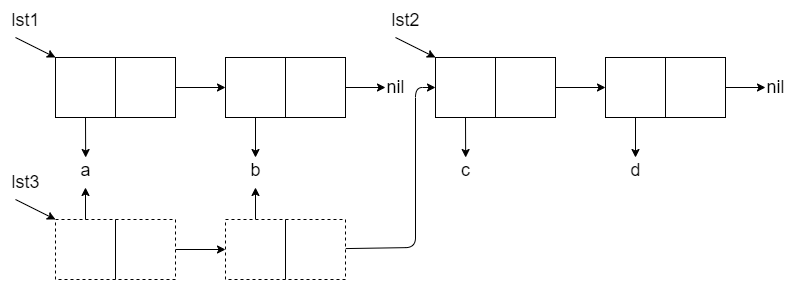
\includegraphics[width=0.9\textwidth]{img/append.drawio.png}
        \label{fig:append-sheme}
    \end{imagebox}
    \caption{Схема работы функции append}
\end{figure}

Работа NCONC аналогична APPEND, только она не создаёт копий,
а переставляет указатели.

\begin{figure}[H]
    \begin{listingbox}{}
        \lstinputlisting[language=Lisp]{lists/nconc.lisp}
    \end{listingbox}
    \caption{Пример работы функции nconc}
    \label{lst:nconc-example}
\end{figure}

\section{reverse и nreverse}

Функции переставляют элементы в обратном порядке.

\begin{figure}[H]
    \begin{listingbox}{}
        \lstinputlisting[language=Lisp]{lists/reverse-nreverse.lisp}
    \end{listingbox}
    \caption{Пример работы функций reverse, nreverse}
    \label{lst:reverse-nreverse-example}
\end{figure}

\section{nth, nthcdr}

NTH возвращает n-нный элемент списка list. Индексация с 0.
NTHCDR выполняет для списка операцию cdr n раз, и возвращает 
результат. Если N больше длины списка, то возвращается nil.
Отрицательное N вызовет ошибку.

\begin{figure}[H]
    \begin{listingbox}{}
        \lstinputlisting[language=Lisp]{lists/nth-nthcdr.lisp}
    \end{listingbox}
    \caption{Пример работы функций nth, nthcdr}
    \label{lst:nth-nthcdr-example}
\end{figure}

\section{last, length}

LAST возвращает последние N ячеек списка. Если N не указано,
возвращается последняя списковая ячейка.

LENGTH возвращает количество списковых ячеек. Может работать 
некорректно на циклических списках.

\begin{figure}[H]
    \begin{listingbox}{}
        \lstinputlisting[language=Lisp]{lists/last-length.lisp}
    \end{listingbox}
    \caption{Пример работы функций last, length}
    \label{lst:last-length-example}
\end{figure}

\section{remove}

REMOVE удаляет все вхождения элемента, указанного первым
параметром, из списка, указанного вторым параметром. По умолчанию
внутри для сравнения элементов используется функция EQL, которая 
не позволяет сравнивать вложенные списки. С помощью оператора 
двоеточие можно явно указать функцию сравнения.

\begin{figure}[H]
    \begin{listingbox}{}
        \lstinputlisting[language=Lisp]{lists/remove.lisp}
    \end{listingbox}
    \caption{Пример работы функции remove}
    \label{lst:remove-example}
\end{figure}

\section{rplaca, rplacd}

Данные функции изменяют соответственно car и cdr элементы 
cons-ячеек первого аргумента-списка на значение второго аргумента,
и возвращают модифицированный первый аргумент.

\begin{figure}[H]
    \begin{listingbox}{}
        \lstinputlisting[language=Lisp]{lists/rplaca-rplacd.lisp}
    \end{listingbox}
    \caption{Пример работы функций rplaca, rplacd}
    \label{lst:rplaca-rplacd-example}
\end{figure}

\section{subst, nsubst}

SUBST выполняет замену в выражении, заданном третьим аргументом 
все вхождения значения второго аргумента НА ВСЕХ УРОВНЯХ на 
значение первого аргумента.

\begin{figure}[H]
    \begin{listingbox}{}
        \lstinputlisting[language=Lisp]{lists/subst-nsubst.lisp}
    \end{listingbox}
    \caption{Пример работы функций subst, nsubst}
    \label{lst:subst-nsubst-example}
\end{figure}

\section{member}

MEMBER осуществляет поиск элемента, удовлетворяющего условию, 
в списке. Если элемент не найдёт, возвращается nil. Иначе 
возвращается часть списка, начинающаяся с искомого элемента.

\begin{figure}[H]
    \begin{listingbox}{}
        \lstinputlisting[language=Lisp]{lists/member.lisp}
    \end{listingbox}
    \caption{Пример работы функции member}
    \label{lst:member-example}
\end{figure}

\section{union, intersection, set-difference}

UNION строит список, содержащий объединение элементов, входящих 
в значения двух ее списков-аргументов.

INTERSECTION возвращает список, состоящий из элементов, входящих 
в оба списка.

SET-DIFFERENCE возвращает набор, содержащий элементы первого списка, 
которые отсутствуют во втором списке.

Все три функции сохраняют неизменными исходные списки.

\begin{figure}[H]
    \begin{listingbox}{}
        \lstinputlisting[language=Lisp]{lists/union-intersection-set-difference.lisp}
    \end{listingbox}
    \caption{Пример работы функций union, intersection, set-difference}
    \label{lst:union-intersection-set-difference-example}
\end{figure}

\section{Ассоциативные таблицы}

Список Lisp можно рассматривать как таблицу: множество точечных пар,
где первый элемент можно воспринимать как ключ, а второй как значение.

\begin{listbox}{\noindent \begin{listboxtitle}{}5\end{listboxtitle} 
	\raisebox{6pt}{Основные функции для работы с таблицами:}}
\begin{enumerate}
	\item pairlis -- принимает два списка и создаёт ассоциативный список, 
    который связывает элементы первого списка с соответствующими 
    элементами второго;
	\item assoc -- возвращает первую пару, удовлетворяющую условию, или nil, 
    если такой пары не было найдено;
	\item rassoc -- реверсивный assoc;
	\item acons -- создаёт новый ассоциативный список, с помощью добавления 
    пары к старому a-list;
	\item sublis --принимает два аргумента. Значением первого аргумента 
    должен быть ассоциативный список. Значением второго 
    аргумента может быть произвольное S-выражение. Функция берет каждый 
    атом, входящий в значение второго аргумента, и заменяет его на 
    ассоциацию из ассоциативного списка. Функция возвращает результат замены.
\end{enumerate}
\end{listbox}

\begin{figure}[H]
    \begin{listingbox}{}
        \lstinputlisting[language=Lisp]{lists/pairlis-assoc-rassoc-acons-sublis.lisp}
    \end{listingbox}
    \caption{Пример работы функций pairlis, assoc, rassoc, acons, sublis}
    \label{lst:pairlis-assoc-rassoc-acons-sublis-example}
\end{figure}